\documentclass[a4paper, 12pt]{article}

\usepackage[margin=1in]{geometry}

%
% Babel package for multiple languages typesetting
%
\usepackage[english]{babel}
\usepackage[T1]{fontenc}
\usepackage[utf8]{inputenc}

%
% One-Half spacing
% Double spacing
%
\usepackage{setspace}
\onehalfspacing
%\doublespacing

%
% Setting the font
%
\usepackage{times}

%
% Rotating tables (e.g. sideways when too long)
%
\usepackage{rotating}


%
% For multiples rows in tables
% 
\usepackage{multirow}

\usepackage{graphicx}
\DeclareGraphicsExtensions{.pdf,.png,.jpg}
\graphicspath{ {./img/} }

\usepackage{caption}
\usepackage{subcaption}

%
% Math packages
% 
\usepackage{amsmath}
\usepackage{mathtools}

%
% Comment and Hyperref
%
\usepackage{verbatim}
\usepackage{hyperref}

\usepackage{natbib}

\usepackage{float}

\usepackage{hyperref}

\newcommand{\HRule}{\rule{\linewidth}{0.25mm}}


\begin{document}

% Design persuasivo de sistemas computacionais: uma abordagem para prever o comportamento do usuário
\begin{titlepage}

\begin{center}

\textsc{\large Final Project}\\[3cm]

\textsc{\large State University of New York - University at Albany}\\[0.5cm]

\textsc{\large PHY/CSI/INF 451/551 - Bayesian Data Analysis}\\[3cm]

% Research Plan Title
\huge Predicting Keywords and Tags of Questions: A Bayesian Data Analysis Approach \\[-0.5cm]
\HRule \\[2cm]

\Large \textbf{Students:} Sibelius Seraphini and Xiaohu Nian \\[0.5cm]

\Large \textbf{Professor:} Kevin H. Knuth 

\vfill

\textbf{2013}

\end{center}

\end{titlepage}


\setlength{\parindent}{0.5in}

\tableofcontents
\newpage
\section{Introduction} \label{sec:introduction}

StackExchange is a collection of 110 questions and answer sites on diverse topics from programming to cooking to photography and gaming. \citep{stackexchange2013site}.
Regarding this, Facebook \citep{facebook2013site} has created an online recruiting competition in Kaggle \citep{kaggle013site} that has the aim of ``Identify keywords and tags from millions of text questions'' \citep{facebook2013keyword}.
Facebook provided a Train and a Test dataset with real questions from the Stack Overflow \citep{stackoverflow2013site}, a StackExchange's site that contain topics from programming languages and computer science.
The task is to predict the tags (a.k.a. keywords, topics, summaries) given only the question text and its title.

Accordingly, a Bayesian Data Analysis was proposed in this project to predict the tags.
With this in mind, the train dataset was used to calculate the prior information, the likelihood values, and the evidence of a given question.



\newpage
\section{Methods and Materials} \label{sec:methods}

The Train set contains 4 columns for each question: Id,Title,Body,Tags.
Id is the unique identifier for each question.
Title is the question's title.
Body is the body of the question.
Tags is the tags associated with the question.
The Test set contains the same columns but without the Tags, which we hava to predict.

Given that our data is text, we employ some text mining techniques \citep{feldman2007text} to transform the data into the prior information, likelihood, and evidence necessary for the bayesian data analysis.

\subsection{Preprocessing the Data}

The first step to analyse this data is to perform some preprocessing (e.g., remove punctuation symbols, all characters to lowercase, and so on).
The steps of our preprocessing approach is showed below:

\begin{enumerate}
    \item One record per line;
    \item Concatenate title and body of questions;
    \item Transform to lowercase;
    \item Remove HTML tags and entities;
    \item Remove Stop Words;
    \item Strip Whitespaces.
\end{enumerate}

The first step aims to remove newlines inside the body questions become only one record per line.
After, we join the title and body of questions to have more change to find keywords.
Next, we transform all the characters to lowercase.
Subsequently, we remove the HTML tags and entities (e.g., <br />, \&lt;), and stop words.
Stop words are common words as \emph{the}, \emph{is}, \emph{at}, \emph{which}; they should be removed to improve the text categorization \citep{silva2003importance}.
Afterwards, we strip the whitespaces, i.e, remove duplicates spaces.
Finally, we reduce our Train set from 6.8 Gigabyte to only 3.9 Gigabyte (\%57); and we reduce our Test set from 2.2 Gigabyte to only 1.3 Gigabyte (\%59).

Preprocessing the data used the \emph{tr} command \citep{ss642013tr}, python and perl. 

\subsection{The Bayesian Data Analysis Approach}

Our Bayesian Data Analysis Approach uses the Bayes' Theorem in formula \ref{eq:bayesian}:

\begin{equation} \label{eq:bayesian}
    P(Tag = t | Keyword = k, I) = \frac{P(Tag = t | I) \times P(Keyword = k | Tag = t, I)}{P(Keyword = k | I)} 
\end{equation}

\begin{enumerate}
    \item $ P(Tag = t | I) $ is the Prior Information about the Tag = t, i.e., what is the probability of a question has a Tag=\emph{t} without any information about this question.
    \item $ P(Keyword = k | Tag = t, I) $ is the Likelihood Probability, that is, the probability of a question has a Keyword = \emph{k} given that question has a Tag = \emph{t}.
    \item $ P(Keyword = k | I) $ is the Evidence, in other words, it is the probability of a Keyword = \emph{k} appear in a question with any Tag.
    \item $ P(Tag = t | Keyword = k, I) $ is the Posterior Probabiity, i.e, the probability of a question has a Tag = \emph{t} given a Keyword = \emph{k}.
\end{enumerate}

The formula \ref{eq:bayesian} can be expanded for any number of keywords, as shows in formula \ref{eq:bayesianMultiples}:

\begin{multline} \label{eq:bayesianMultiples}
    P(Tag = t | Keywords = \{k_{1},k_{2}, \dots , k_{n}\} , I) =  \\
    \frac{P(Tag = t | I) \times P(Keyword = \{k_{1},k_{2}, \dots , k_{n}\} | Tag = t, I)}{P(Keyword = \{k_{1},k_{2}\}, \dots , k_{n}} | I) 
\end{multline}

\subsection{From the Trainset to the Probabilities}

This subsection describe the approach to calculate the Prior Information, the Likelihood, and the Evidence using the dataset provided in the Trainset.

The Prior Information of a given Tag=\emph{t} was defined as the frequency of the Tag in the trainset, i.e., the number of questions that has the Tag=\emph{t} divided by the total number of question in the trainset; the formula \ref{eq:prior}

\begin{equation} \label{eq:prior}
    P(Tag = t | I) = \frac{\text{Number of questions of Tag=t}}{\text{Total number of questions in the trainset}}
\end{equation}

The Likelihood Probability of a Keyword=\emph{k} given a Tag=\emph{t} is the importance value of the keyword divided by the sum of importance of the other keywords in questions that have Tag=\emph{t}.
The importance of a keyword is calculate using the Tf-Idf, a numerical statistic that reflects how important a word is to a document in a collection of documents \citep{aizawa2003information}.
Keywords are the words that best describe a Tag (a.k.a. keywords, topics, summaries).
It was selected the 20 most important word to be the keywords of a given tag.
The formula \ref{eq:likelihood} illustrate this calculation.
Additionally, the formula \ref{eq:likelihoodMult} show how to expand it to a set of keywords.

\begin{equation} \label{eq:likelihood}
    P(Keyword=k | Tag=t, I) = \frac{\text{Importance value of the Keyword \emph{k}}}{\text{Sum of Importance of the other Keywords of Tag=\emph{t}}}
\end{equation}

\begin{multline} \label{eq:likelihoodMult}
    P(Keyword=\{k_{1},k_{2}, \dots , k_{n}\} | Tag=t, I) = \\
    \prod_{k \: \in \: \{k_{1},k_{2}, \dots , k_{n}\}} P(Keyword=k | Tag=t,I)
\end{multline}

The Evidence is calculate using the Prior Information of all the Tags and the Likelihood of all the combination of keywords and tags.
The formula \ref{eq:evidence} show that how to calculate the Evidence given the Prior Information and the Likelihood.
The formula \ref{eq:evidenceMult} expands to a set of keywords.

\begin{equation} \label{eq:evidence}
    P(Keyword=k | I) = \sum_{t \: \in \: Tags} P(Keyword=k | Tag=t, I) \times P(Tag=t | I)
\end{equation}

\begin{multline} \label{eq:evidenceMult}
    P(Keyword=\{k_{1},k_{2}, \dots , k_{n}\} | I) = \\
    \sum_{t \: \in \: Tags} \prod_{k \: \in \: \{k_{1},k_{2}, \dots , k_{n}\}} P(Keyword=k | Tag=t,I) \times P(Tag=t | I) 
\end{multline}

In summary, this subsection described how to calculate the Prior Information, the Likelihood, and the Evidence using the Trainset.
Hence, it is possible to calculate the Posterior Probability using the keywords of a question.




\newpage
\section{Results} \label{sec:results}

The evaluation of the Bayesian Data Analysis approach proposed used a small set of the trainset.
This small set contains 20000 questions preprocessed of the tags: \emph{java}, \emph{android}, \emph{php}, and \emph{c++}.
5000 questions of each tag.

The Prior Information calculated for the four tags is shown in Figure \ref{fig:prior}.
The most probable tag is \emph{java} with 0.31.

The Figure \ref{fig:likelihood} contains four figures that show the likelihood for the first five keywords for the four tags.
It is worth mentioning, there are keywords that appear in more than one tag, for instance, the keyword \emph{file} is one of the top five keywords for \emph{c++}, \emph{java}, and \emph{php}.

For the evaluation with consider that one question has only one tag.
The experiment used from 1 top keyword to 20 top keywords.
The Figure \ref{fig:accuracy} shows the accuracy for these experiments.
The best result using the Bayesian Data Analysis approach was using 1 top keyword (73\% of hits), and using 5 top keywords (61 \% of hits).

\begin{figure}[ht]
    \centering
    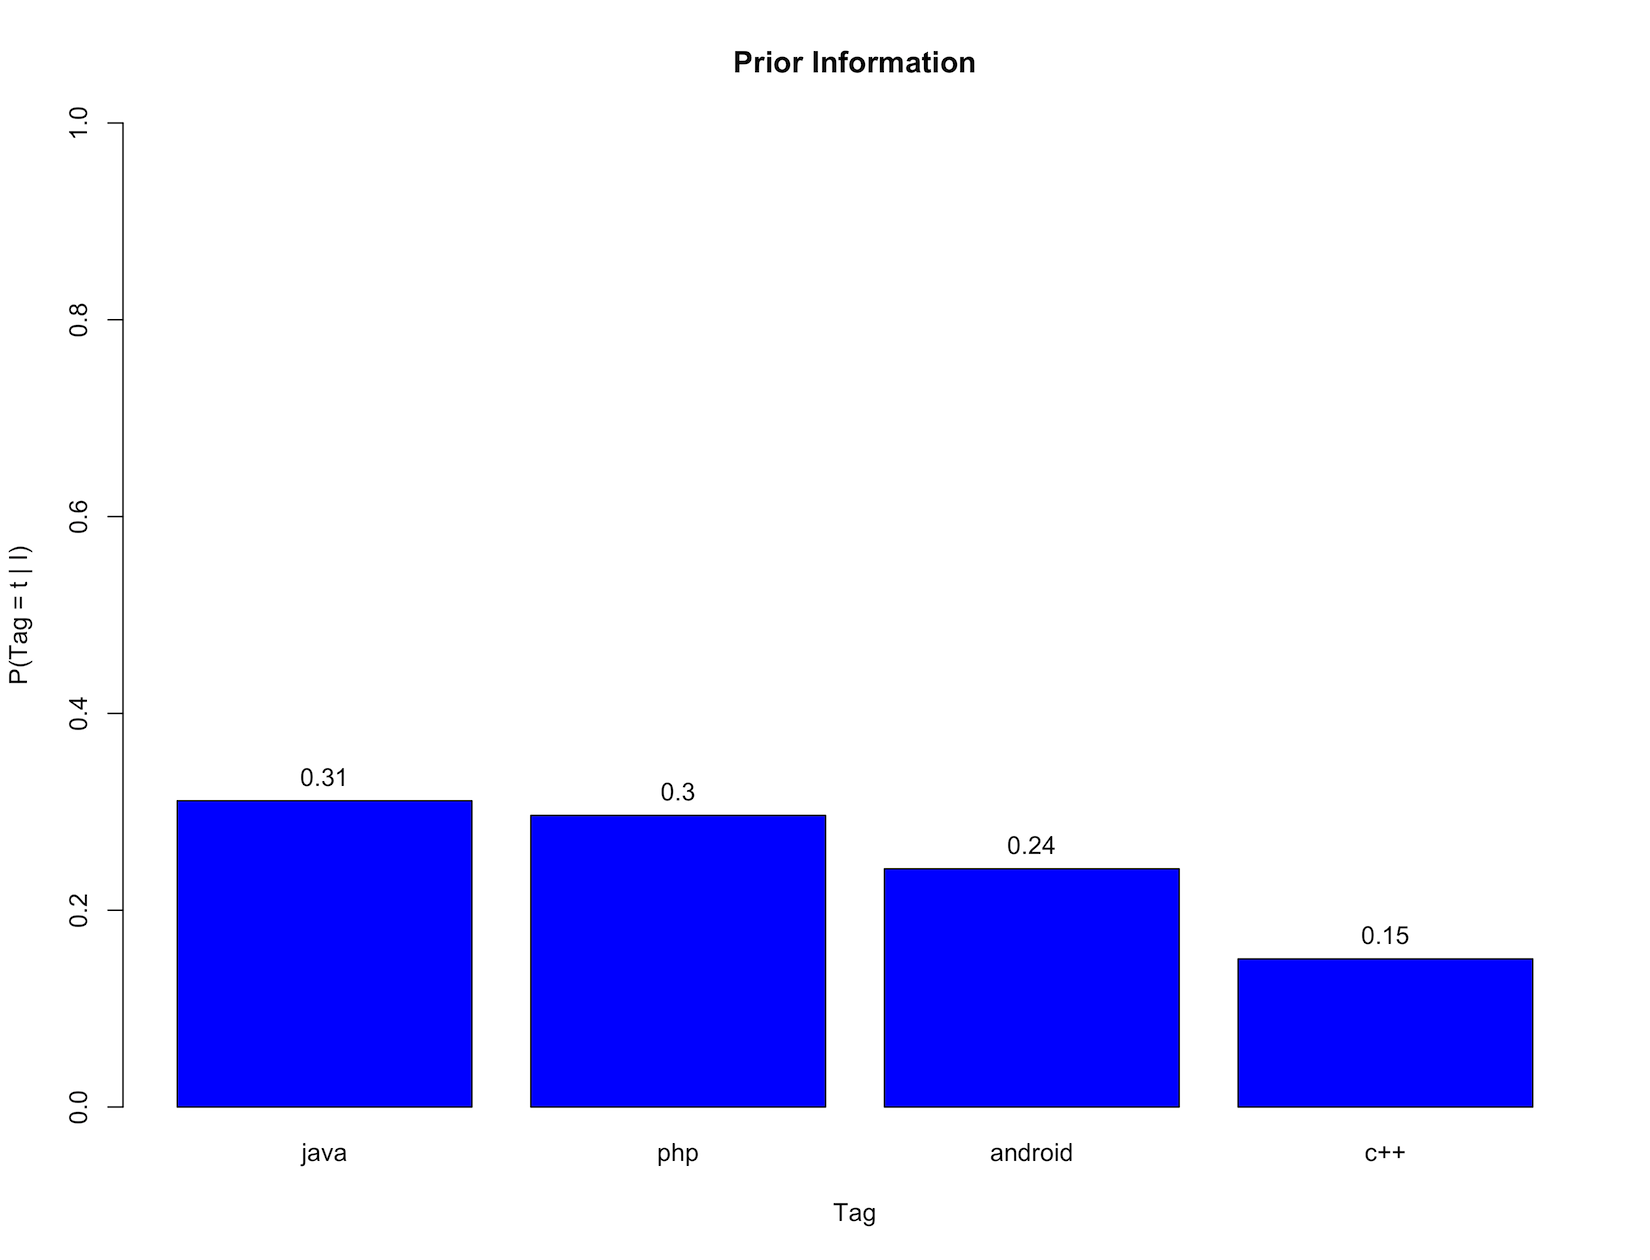
\includegraphics[scale=0.4]{prior}
    \caption{Prior Information}
    \label{fig:prior}
\end{figure}

\begin{figure}[H]
    \centering
    \begin{subfigure}[b]{.40\textwidth}
        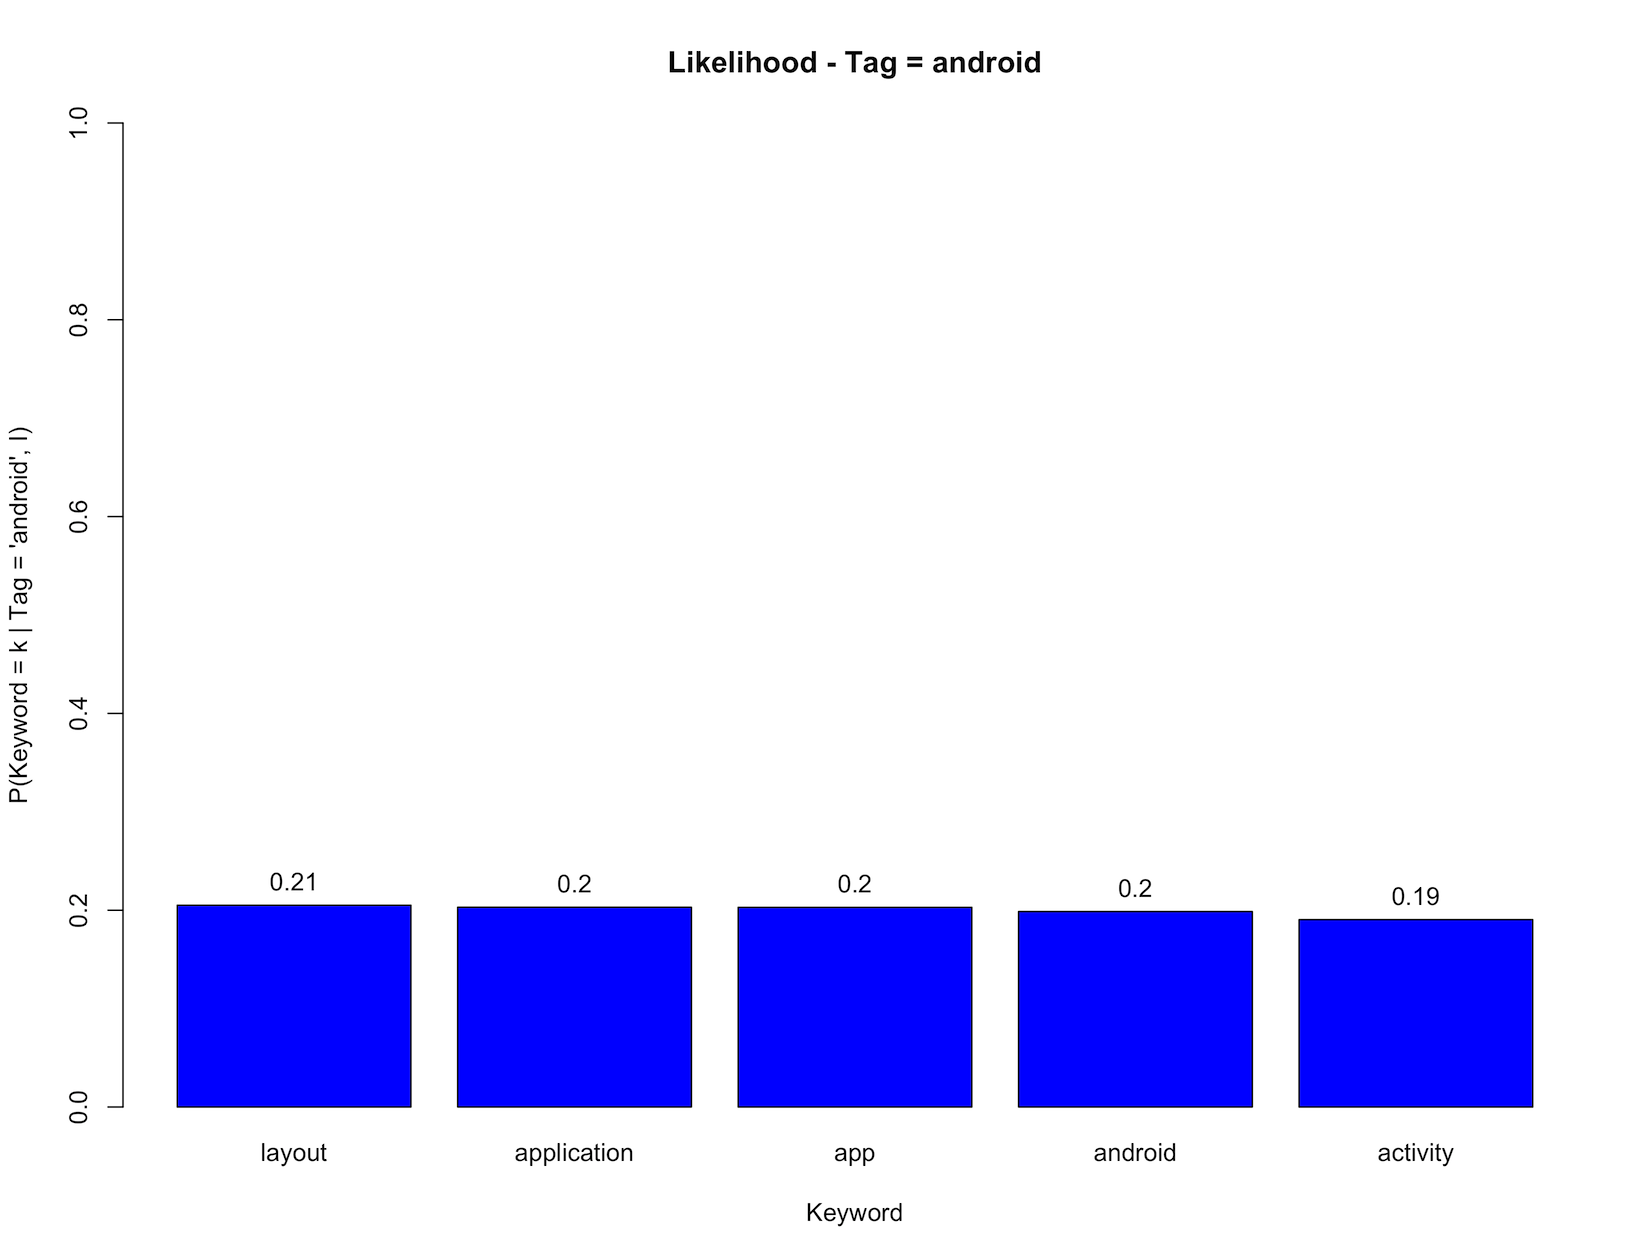
\includegraphics[width=\textwidth]{likelihood_android}
        \caption{Likelihood Android}
        \label{fig:likelihood_android}
    \end{subfigure}
    \begin{subfigure}[b]{.40\textwidth}
        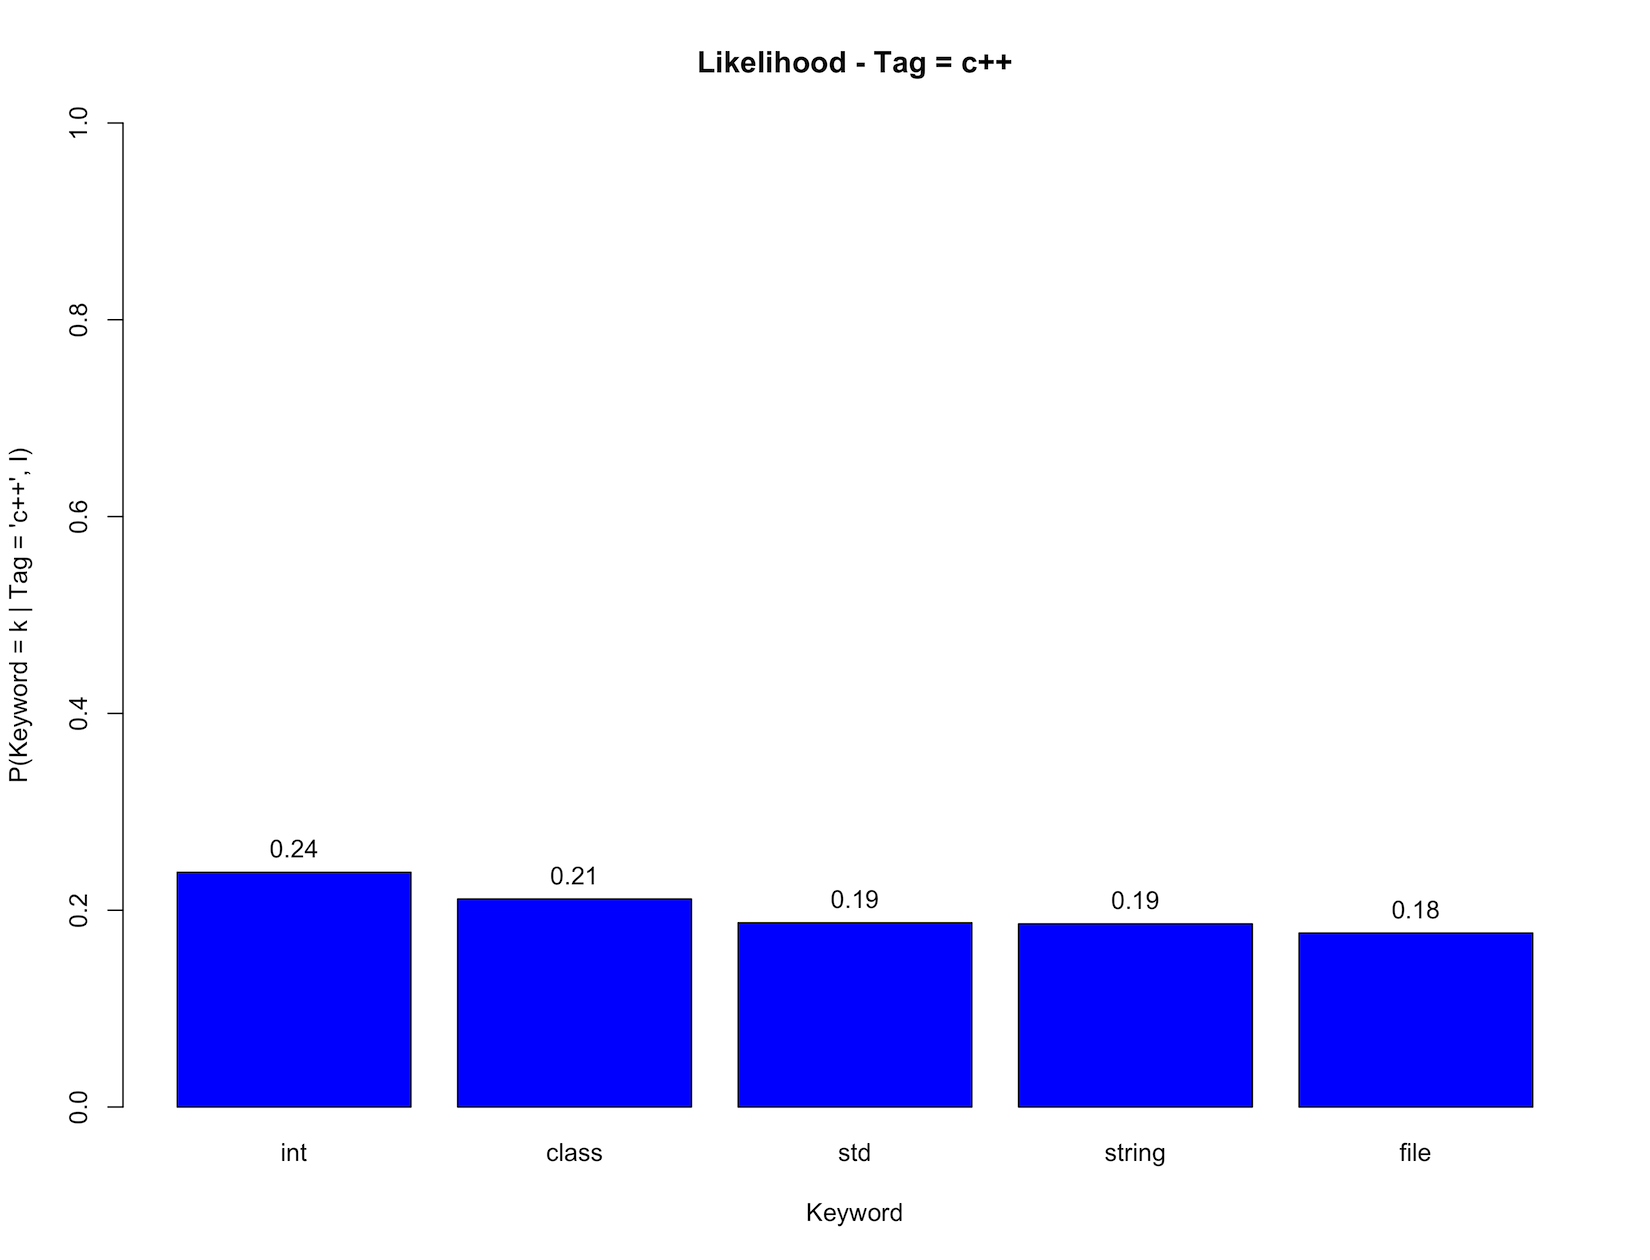
\includegraphics[width=\textwidth]{likelihood_c++}
        \caption{Likelihood C++}
        \label{fig:likelihood_c++}
    \end{subfigure}
    \begin{subfigure}[b]{.40\textwidth}
        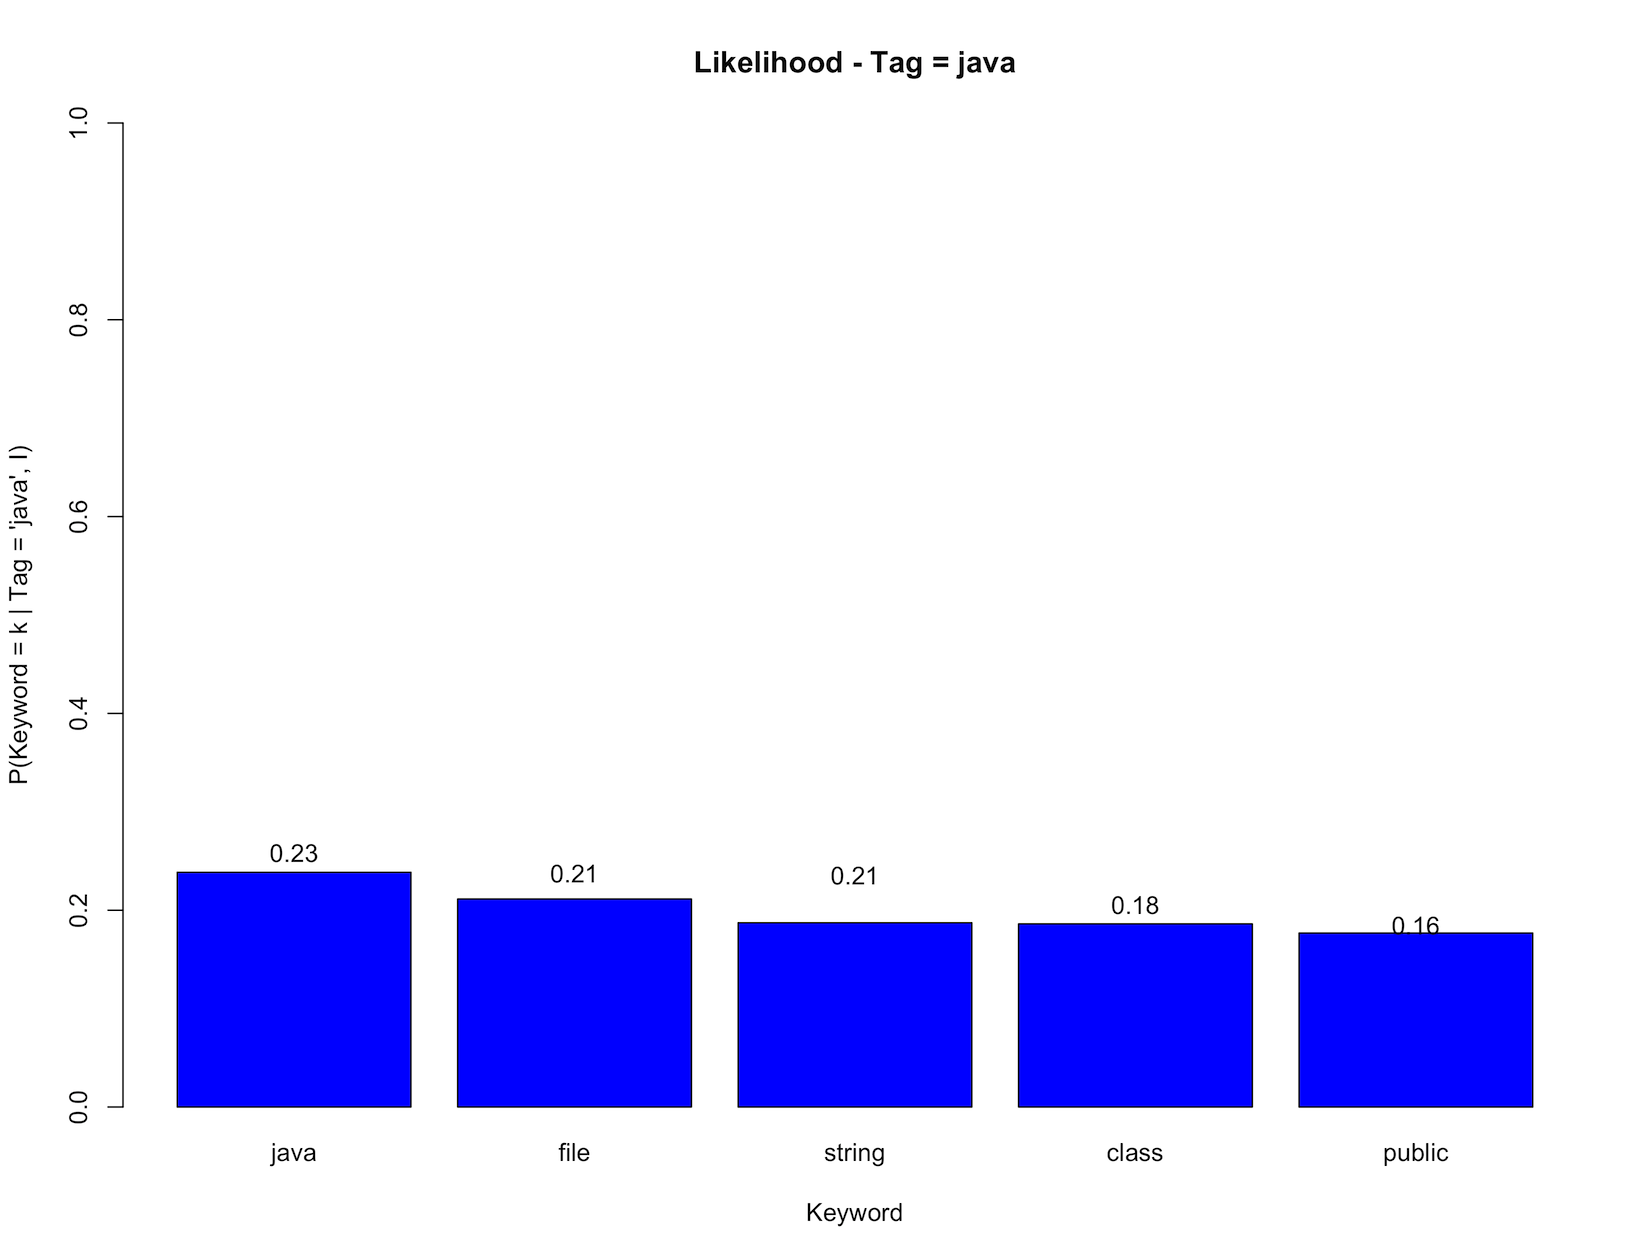
\includegraphics[width=\textwidth]{likelihood_java}
        \caption{Likelihood Java}
        \label{fig:likelihood_java}
    \end{subfigure}
    \begin{subfigure}[b]{.40\textwidth}
        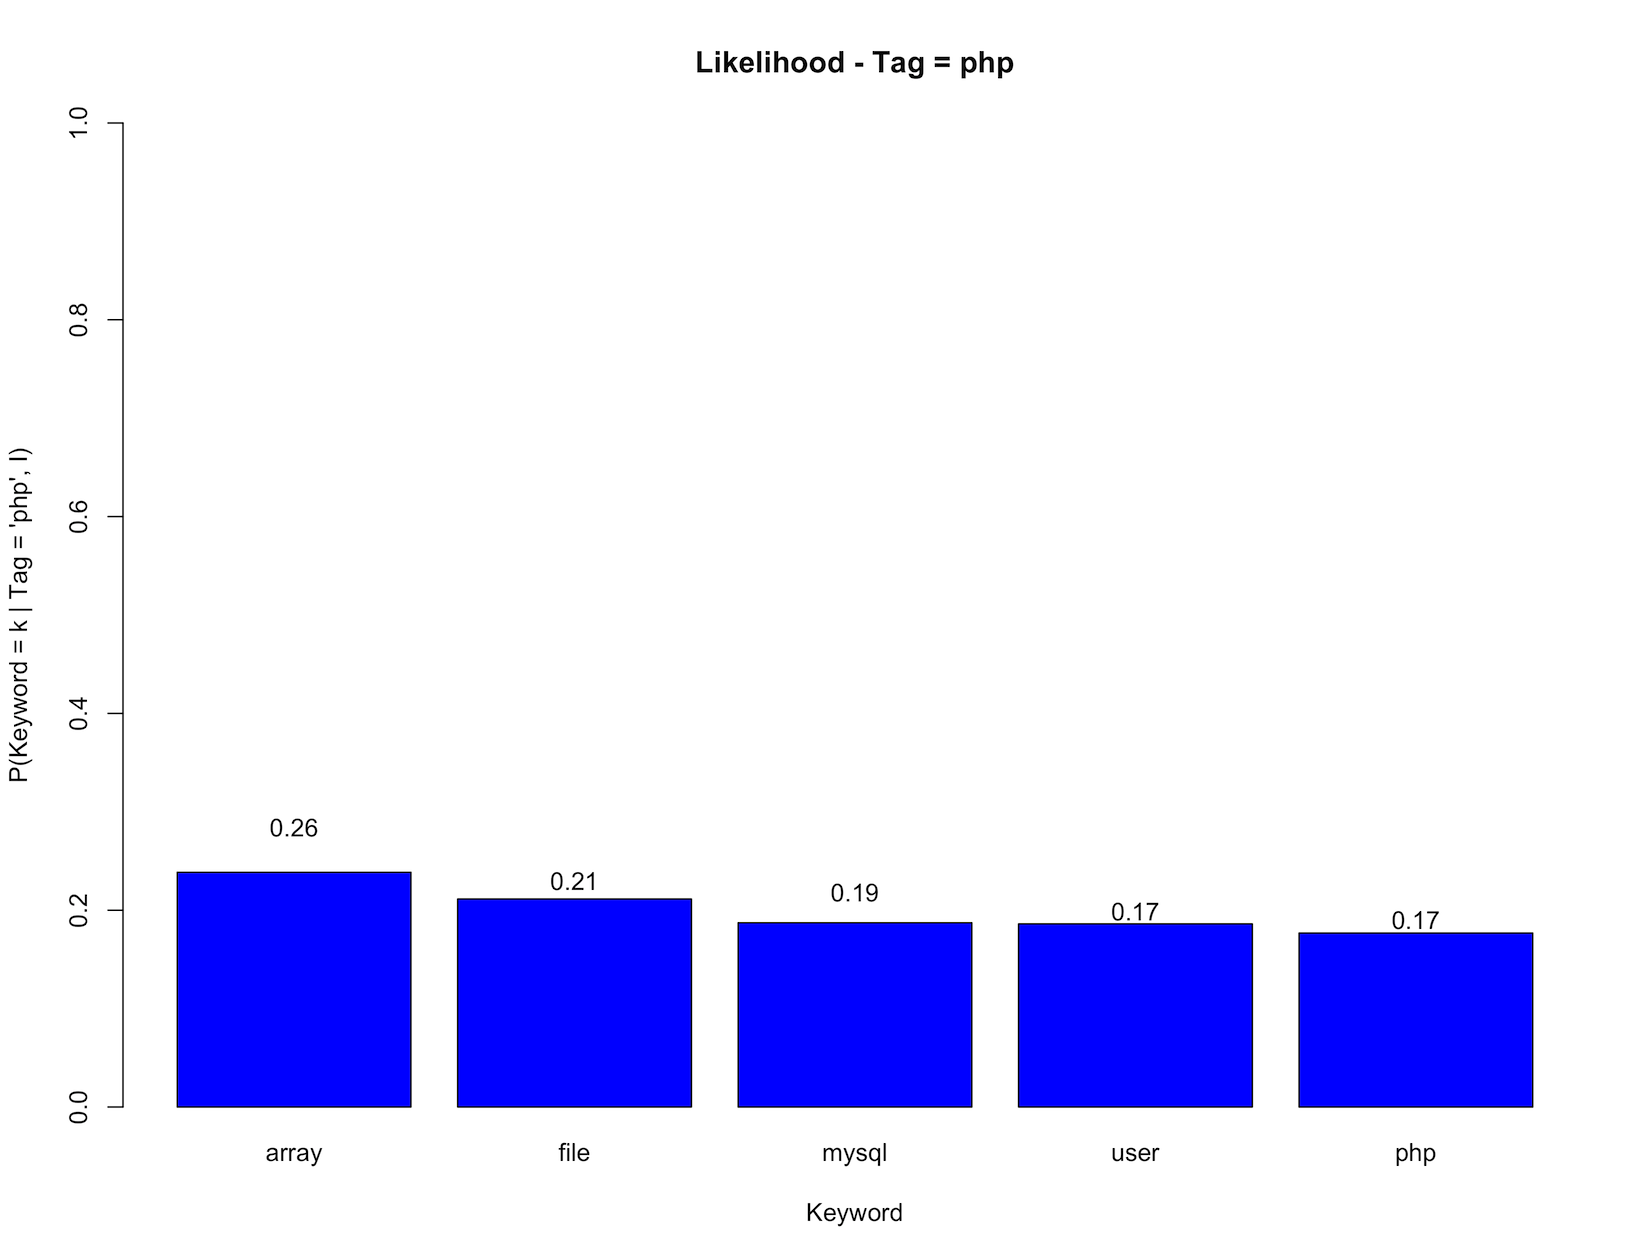
\includegraphics[width=\textwidth]{likelihood_php}
        \caption{Likelihood Php}
        \label{fig:likelihood_php}
    \end{subfigure}
    \caption{Likelihood}
    \label{fig:likelihood}
\end{figure}

\begin{figure}[H]
    \centering
    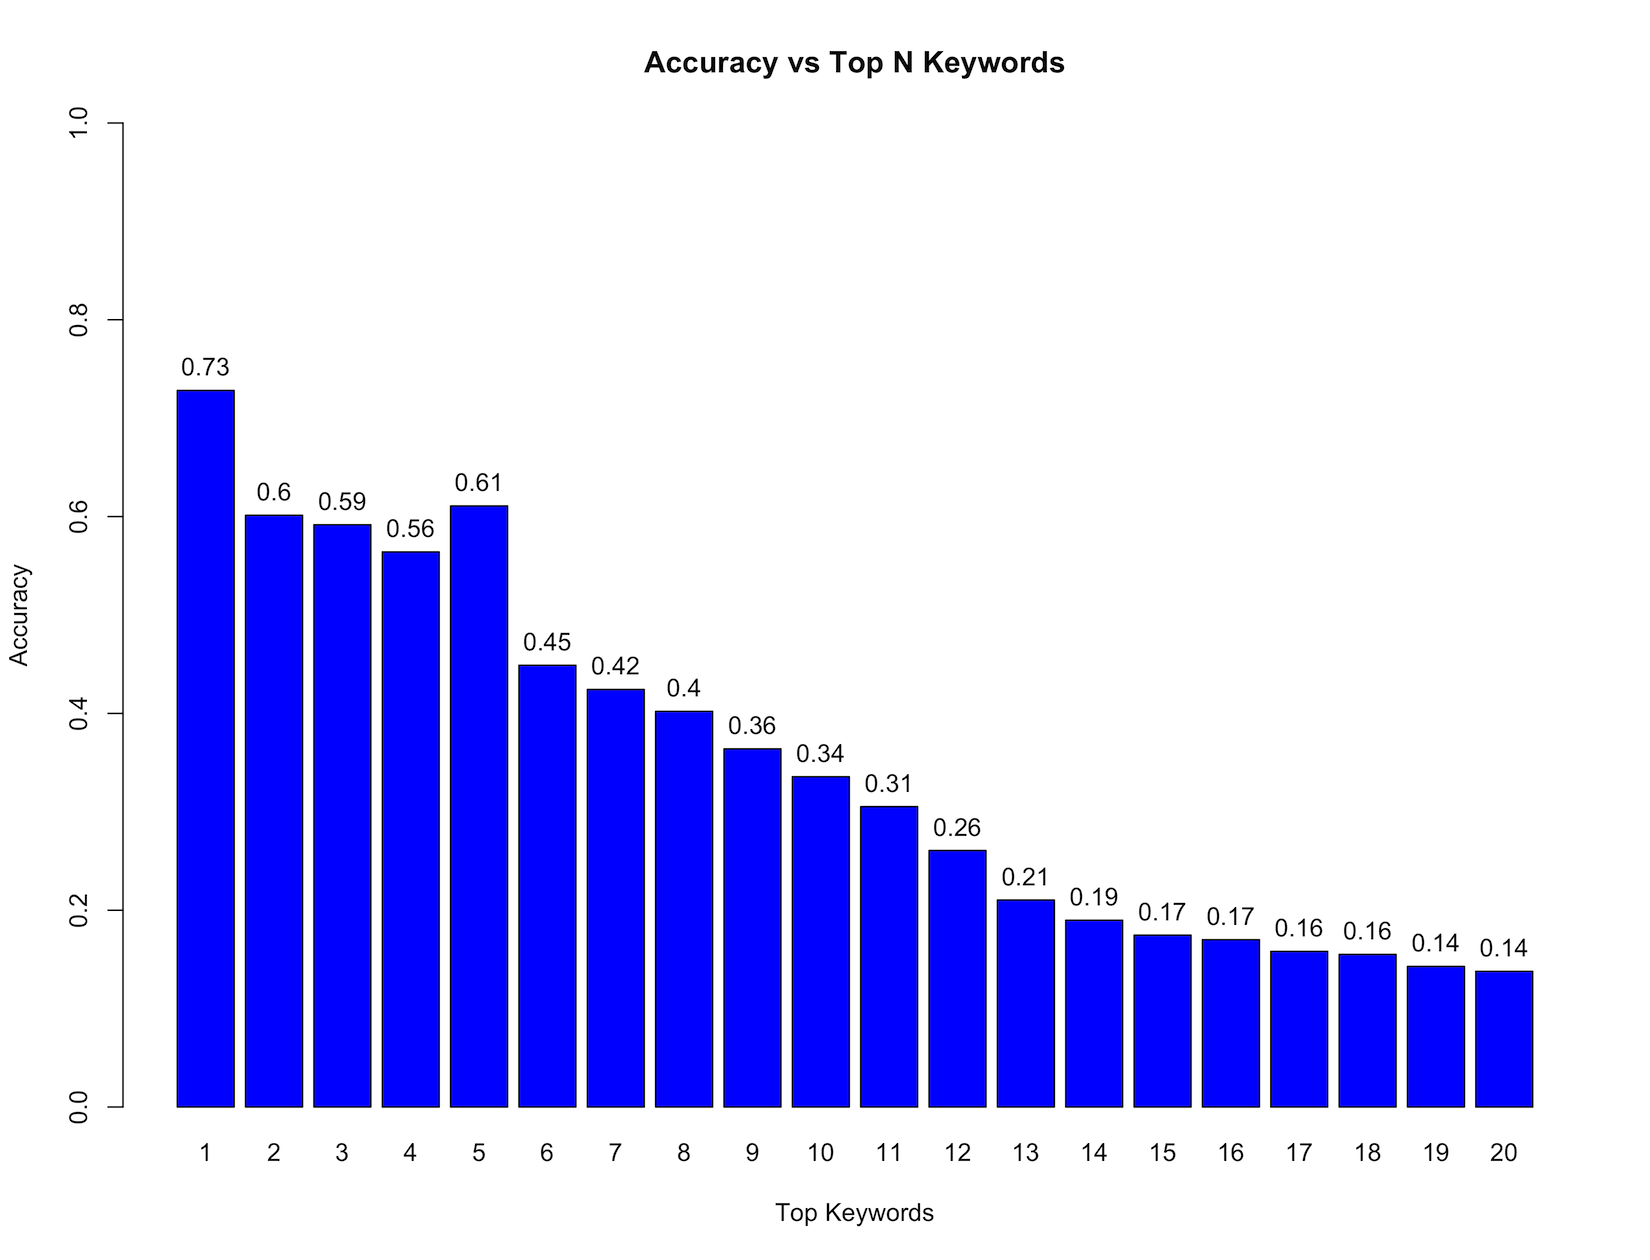
\includegraphics[scale=0.4]{accuracy}
    \caption{Comparison between difference optimization approaches}
    \label{fig:accuracy}
\end{figure}


\newpage
\section{Conclusion} \label{sec:conclusion}
The Bayesian model assumes the independence between keywords. However, in most cases keywords happen to cooccur. The model we use may lead to some error induced by the assumption of independence. In order to correct this type of error, future work can be done about how to use train dataset to deduce the cooccurrence and incorporate this type of information into the prior knowledge to get more accurate predication of tags. Besides that, the model is limited because we already chose the tags. In order to make the model work in practice, we need to figure out a method to choose the set of the most possible candidate tags, and thus reduce the computation cost.

As for the reason why we choose R over Matlab lies on the fact that R is open source and it has a richer text mining ability to further the future work.


\newpage
\bibliographystyle{apalike}
\bibliography{bibliography}

\end{document}

